\documentclass[12pt,aspectratio=169,hyperref={pdftex,unicode},xcolor=dvipsnames]{beamer}
\usepackage[english]{babel}
\usepackage[utf8x]{inputenc}
\usepackage[T2A]{fontenc}
\usepackage{cmap}
\usepackage{paratype}
\usepackage{minted}
\usepackage{blkarray} % for examples with code (require parameter -shell-escape)

\usetheme{metropolis}
\usefonttheme[]{professionalfonts}  % prohibit overwriting fonts to beamer
\metroset{numbering=fraction}
\metroset{subsectionpage=progressbar}

\setbeamercolor{frametitle}{fg=black}
\setbeamertemplate{frametitle}
{
    \vspace{3mm}\insertframetitle\par
}
\setbeamertemplate{title separator}{}
\setbeamertemplate{footnote separator}{}

\logo{\vspace{-1.2cm}
\includegraphics[width=8mm]{./common/nup-icon.png}\hspace*{1.08\textwidth}}

\institute
{
    \begin{columns}
        \begin{column}{2.5cm}
            \includegraphics[height=30mm,keepaspectraticommon/nup-icon.png]
        \end{column}
        \begin{column}{3cm}
            Neapolis University Paphos
        \end{column}
    \end{columns}
}

\begin{document}

    \begin{frame}[plain]
        \begin{left}

        {\Large\textbf{Here is The Topic of Your Bachelor's Thethis: It's a Minimum Two-Line Title}}

            \vspace{5mm}
            \textbf{Your First Name and Last Name}

            {\small Supervisors: A.\,Ivanov, B.\,Georgiou}

            \vspace{10mm}
            DATE
        \end{left}

        \vspace{10mm}

        \begin{column}{1cm}
            
\includegraphics[height=14mm,keepaspectratio]{./common/nup-logo.png}
        \end{column}
    \end{frame}



    \begin{frame}
        \frametitle{Introduction to The Subject Area\footnote{By the way, slides with long enumerations look bad. Try to avoid them.}}

        \begin{itemize}
            \item What is the thesis about?
            \item Why is it useful?
            \item Who else is working on this? Are there any analogs?
            \item This slide is necessary to make the problem statement clearer.
            \item We advice to make no more than two slides like this, otherwise, you won't have enough time to talk about your work.
            \item The introduction to The Subject Area should take no more than 15\% of your presentation time.
        \end{itemize}


    \end{frame}

    \begin{frame}
        \frametitle{The Problem Statement}
        \begin{enumerate}
            \item What task were you trying to solve?
            \item ...
        \end{enumerate}
    \end{frame}

    \begin{frame}{Task 1: Formula with Explanations}
        The filter minimizes the standard deviation of the pixel color.

        \begin{equation*}\label{eq:wiener_nsr}
        \hat{Y}(i, j) = \left[ \frac{\hat{H}^*(i, j)}{\left|\hat{H}(i, j)\right|^2 + \frac{S_n(i, j)}{S_s(i, j)}} \right] \times \hat{F}(i, j),
        \end{equation*}
        \begin{itemize}
            \item $Y$ -- restored image,  $F$ -- observed image,
            \item $H$ -- scattering function, $H^*$ -- complex conjugate $H$,
            \item $S_n$ -- energy spectrum of the noise -- $\left| \hat{N} \right|^2$,
            \item $S_s$ -- energy spectrum of the source image -- $\left| \hat{F} \right|^2$,
            \item $\times$ -- multiplication of complex numbers.
        \end{itemize}
    \end{frame}

    \begin{frame}[fragile]
        \frametitle{Task 2: Сode\footnote{Be careful with the code on the slides, it is better to give preference to diagrams and tables.}}
        \begin{minted}{kotlin}
fun main() {
    val name = "stranger"
    println("Hi, $name!")
    print("Current count:")
    for (i in 0..10) {
        print(" $i")
    }
}
        \end{minted}
    \end{frame}

    \begin{frame}{Task 2: Results in Table}
        \centering
        \begin{tabular}{lccc}
            Name & Score 1 & Score 2 & Result \\
            \hline\hline
            Alice & 8.0 & 9.0 & 8.5 \\
            Bob & 9.0 & 9.8 & 9.4 \\
            Chak & 9.1 & 9.3 & 9.2 \\
        \end{tabular}

        \begin{block}{Table Notes}
            \begin{itemize}
                \item Tables may require explanations.
                \item What are these values? Where did they come from?
                \item What conclusions can be done?
            \end{itemize}
        \end{block}

    \end{frame}


    \begin{frame}
        \frametitle{Task 2: Сomparison with Сompetitors\footnote{Is your diagram clear? Have you forgotten the legend?}\footnote{Is the image contrasting? Things can look worse on the projector.}}
        \begin{center}
            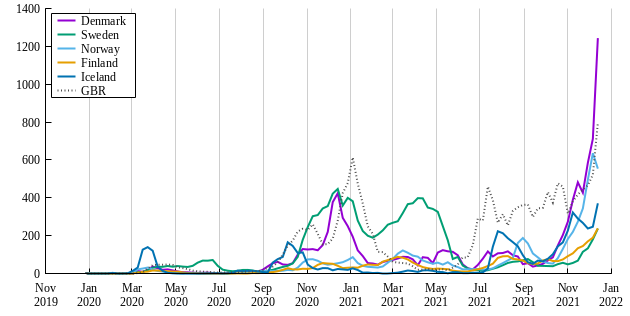
\includegraphics[width=11cm]{images/graph.png}
        \end{center}
    \end{frame}

    \begin{frame}
        \frametitle{Extra Slide}
        \begin{itemize}
            \item Information about the implementation
            \item Future plans (it's better to be realistic:)
            \item References to the literature --- can be placed at the end of the slides, but not shown during the presentation.
            \item Abbreviations. We recommend to use only widely accepted and well-known ones.
        \end{itemize}

    \end{frame}


    \begin{frame}
        \frametitle{Results}

        \begin{enumerate}
            \item A polynomial algorithm for solving the traveling salesman problem has been developed.
            \item The software implementation demonstrates the highest performance and surpasses all known analogues.
            \item The results have been prepared for the report at the conference ~FOCUS.
        \end{enumerate}

        \vspace{5mm}\hrule\vspace{5mm}

        \begin{center}
            First name, Last name and Contacts of the Author,\\link to the materials, QR-code.
        \end{center}

    \end{frame}

    \begin{frame}[noframenumbering,plain]
        \begin{center}
            \Huge Thank you!

                {\color{red}You don't need this slide! It's better to delete it. \footnote{And it's better to delete the footnotes on the slides too. It's possible to say a lot just in words.}}
        \end{center}

    \end{frame}

\end{document}
